
\section{\ttd\ Jet Multiplicity Reweighting Procedure Information}
\label{app:ttdlnj}


\begin{figure}[hbt]
  \begin{center}
	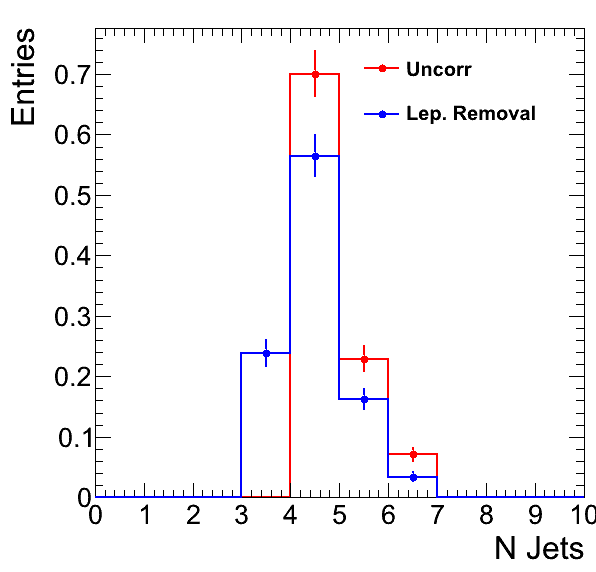
\includegraphics[width=0.5\linewidth]{plots/ttdl_njets_lepremoval_comp.png}
	\caption{
	  \label{fig:dileptonnjets_lepcomp}%\protect 
          Comparison of the jet multiplicity distribution for \ttll\
          events in MC in the signal sample before (red) and after
          (blue) applying the lepton-jet overlap removal. Note only
          the first 6 jets are shown.}  
      \end{center}
\end{figure}


In the signal sample, leptons mis-identified as jets are not rare. 
Figure~\ref{fig:dileptonnjets_lepcomp}  shows the MC jet
multiplicity distribution for \ttll\ events satisfying the full
selection criteria before and after subtracting leptons mis-identified
as jets. Approximately a quarter of the sample is comprised of 4-jet
events that actually correspond to a 2-lepton + 3 jet event where the second
lepton is counted as a jet. Lepton mis-identification depends strongly
on the type of second lepton, occuring more frequently in the case of
hadronic $\tau$s than leptonic objects. According to the \ttll\
MC, for hadronic $\tau$s, $\sim85\%$ of multi-prong $\tau$s and about half
the single-prong $\tau$ are mis-identified as jets. In the case of
leptonic objects, the fractions are smaller, comprising about a third
of \E/\M\ from a \W\ decay and $<20\%$ for leptonic $\tau$s, 
mainly because of the softness of the decay products. 
The scale factors listed in Table.~\ref{tab:njetskfactors} are applied
to the ``cleaned'' jet counts in the signal sample (shown in blue in
Figure~\ref{fig:dileptonnjets_lepcomp}). The impact of applying the
jet multiplicity scale factors on the \ttll\ is about a $10\%$ reduction in the
background prediction for the signal region. 

%\begin{itemize}
%\item Hadronic ($\tau$) objects: most multi-prong $\tau$s and about
%  half single-prong $\tau$s 
%\item Leptonic objects: smaller fraction, 
%\end{itemize}
%Fraction of various lepton types matched to a jet
%multi-prong taus ⟹ 85% give additional 30 GeV jet
%single-prong taus ⟹ ~50% give additional 30 GeV jet
%leptonic taus ⟹ <20% give additional 30 GeV jet
%e/mu⟹ ~40% give additional 30 GeV jet 

\begin{figure}[hbt]
  \begin{center}
	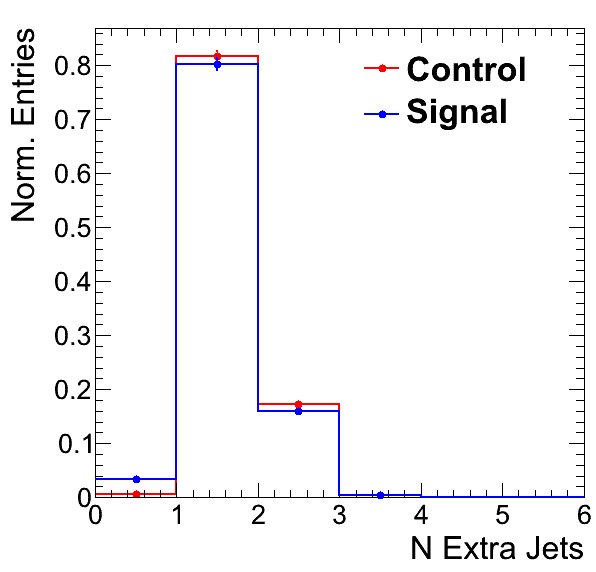
\includegraphics[width=0.5\linewidth]{plots/ttdl_njets_presel_3j_comp.png}%
	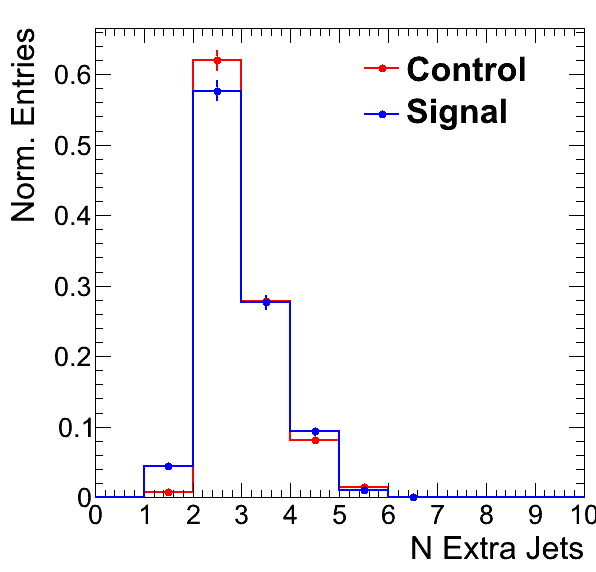
\includegraphics[width=0.5\linewidth]{plots/ttdl_njets_presel_4j_comp.png}
	\caption{
	  \label{fig:dileptonnjets_signalcontrol_comp}%\protect 
          Comparison of the number of additional jets from radiation
          in the 3-jet (left) and $\ge4$-jet (right) bins for the control \ttll\
          sample (with two reconstructed leptons) and the signal
          sample (with one reconstructed lepton). The distributions
          show good agreement, indicating that the usage of the
          reconstructed jet multiplicity in one sample to reweight the
        signal sample is indeed justified. {\bf Fix me: Is this before or after the isolated track veto?}}  
      \end{center}
\end{figure}

Ultimately, the interesting quantity for reweighting is the number of
additional hard jets from radiation and this information is accessed using the
number of reconstructed
jets. Figure~\ref{fig:dileptonnjets_signalcontrol_comp} 
demonstrates in MC that the \ttll\ control sample, i.e. when both leptons are reconstructed,
can indeed be used to reweight the \ttll\ signal sample, i.e. when one lepton is missed.
The figure compares the
number of additional jets from truth matching probed by N
reconstructed jets, in this case 3 and $\ge4$ jets. In order to do so,
jets that are truth-matched to the top decay products (the b-quarks
and additional leptons) are removed. The 3-jet distribution shows 
excellent agreement and the differences in the $\ge4$-jet distribution 
are at most $5\%$. The impact of possible differences in the
underlying distribution of extra
jets between the signal and control \ttll\ samples are estimated by
varying the scale factor contributions by $10\%$ and calculating the
change in the dilepton prediction. This effect is found to have a
negligible impact on the prediction, well below $1\%$.

Other effects that have been examined include the impact of 
additional jets from pileup that may bias the jet multiplicity
distribution, which  is found to be a negligible effect in this dataset. The
impact of the non-\ttll\ background on the jet fraction scale factors
has also been studied. In particular, given the large uncertainty on
the $\dy+HF$ MC prediction, this component has been varied by a factor
of 2 and the resulting change on the dilepton prediction is $<1\%$. As
a result, the dominant source of uncertainty is the statistical
uncertainty, primarily from the two-lepton control sample size, that
corresponds to a $3\%$ uncertainty on the dilepton prediction. 

The scale factors for the fraction of additional jets in the dilepton
sample are applied throughout the analysis. It may be noted that this
scaling is also performed consistently for the alternative \ttbar\
samples, always reweighting the jet multiplicity distribution to the
data in the \ttll\ control sample. In this way, effects truly
arising from using different MC samples and settings can be examined,
separately from issues related to the modeling of additional jets. 


